\chapter{Using sidBison}

This section presents a small example of using \verb|sidBison|. Given a \verb|Flex| file \verb|lexer.l|, and a \verb|Bison| file \verb|parser.y|, a lexer shared object  \verb|lex.so| can be prepared for input to \verb|sidBison| as follows:

\begin{Verbatim} [frame=single]

ibison -d parser.y
flex lexer.l   
gcc -c -fPIC lex.yy.c
gcc -shared -o lex.so lex.yy.o

\end{Verbatim}

This requires the \verb|LD_LIBRARY_PATH| environment variable to include the directory in which \verb|lexer.so| is available and the \verb|BISON_PKGDATADIR| variable points to the \verb|ibison\data| directory. \verb|sidBison| can now be run with \verb|parser.y| and \verb|lex.so| as command-line arguments.

\section{Lambda Calculus}

The lambda calculus example described in Appendix B involves files \href{https://github.com/sidprasad/sidbison/blob/master/lambdacalcexample/lambdacalc.l}{lambdacalc.l} and \href{https://github.com/sidprasad/sidbison/blob/master/lambdacalcexample/lambdacalc.y}{lambdacalc.y}.

\paragraph{Compilation} These files can be compiled to create a lexer shared object file for input for \verb|sidBison| as described below..

\begin{Verbatim} [frame=single]

ibison -d lambdacalc.y
flex lambdacalc.l   
gcc -c -fPIC lex.yy.c
gcc -shared -o lex.so lex.yy.o

\end{Verbatim}

After compilation, the generated files can be loaded into \verb|sidBison| as command line arguments.

\begin{Verbatim} [frame=single]

./sidbison lambdacalc.y lex.so

\end{Verbatim}

\subsection{Debugging input}

The file \href{https://github.com/sidprasad/sidbison/blob/master/lambdacalcexample/input/ycombinator.err} {ycombinator.err} contains the string \verb|\h.(\h.(\x.(h (x x))) \x.(h (x x)))|. This is not accepted by the specified lambda calculus grammar. An example step-through debug is described below.\\



\begin{figure}[H] \centering
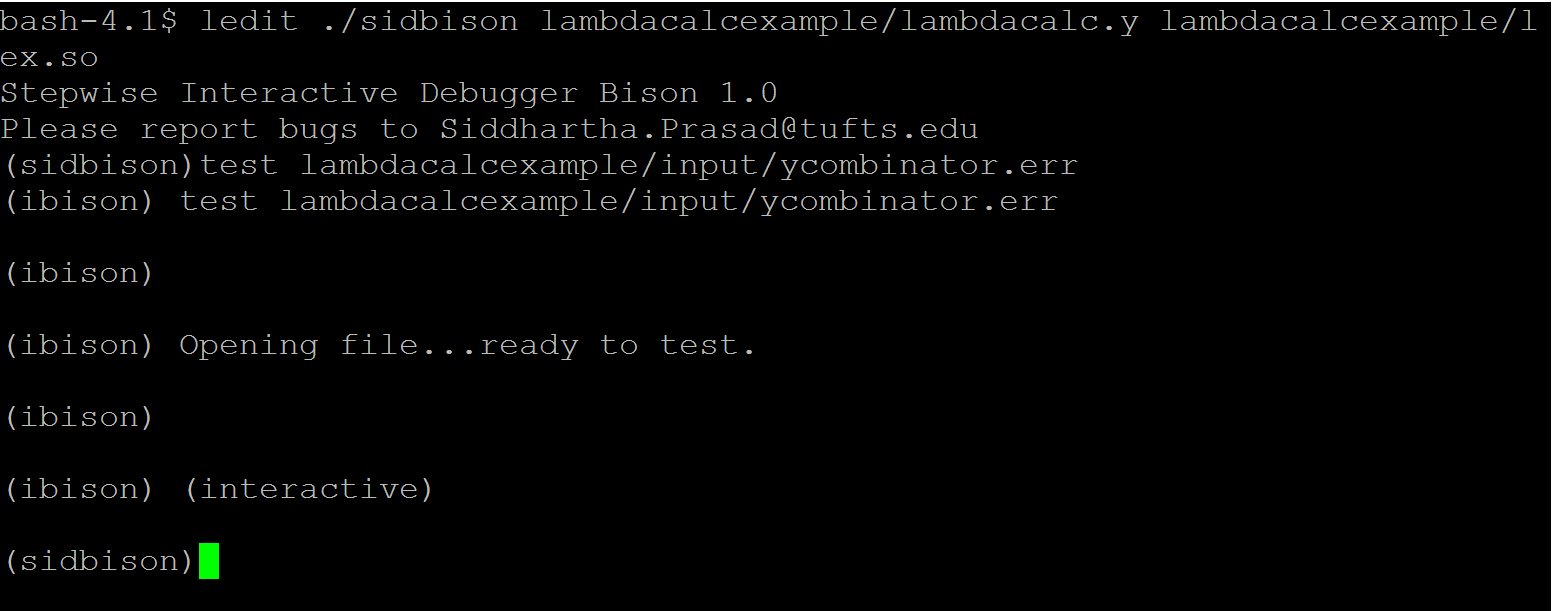
\includegraphics[width=10cm]{lc_1.png}
\end{figure}

\noindent

\verb|ycombinator.err| was loaded into \verb|sidBison| using the \verb|test| command.

\begin{figure}[H] \centering
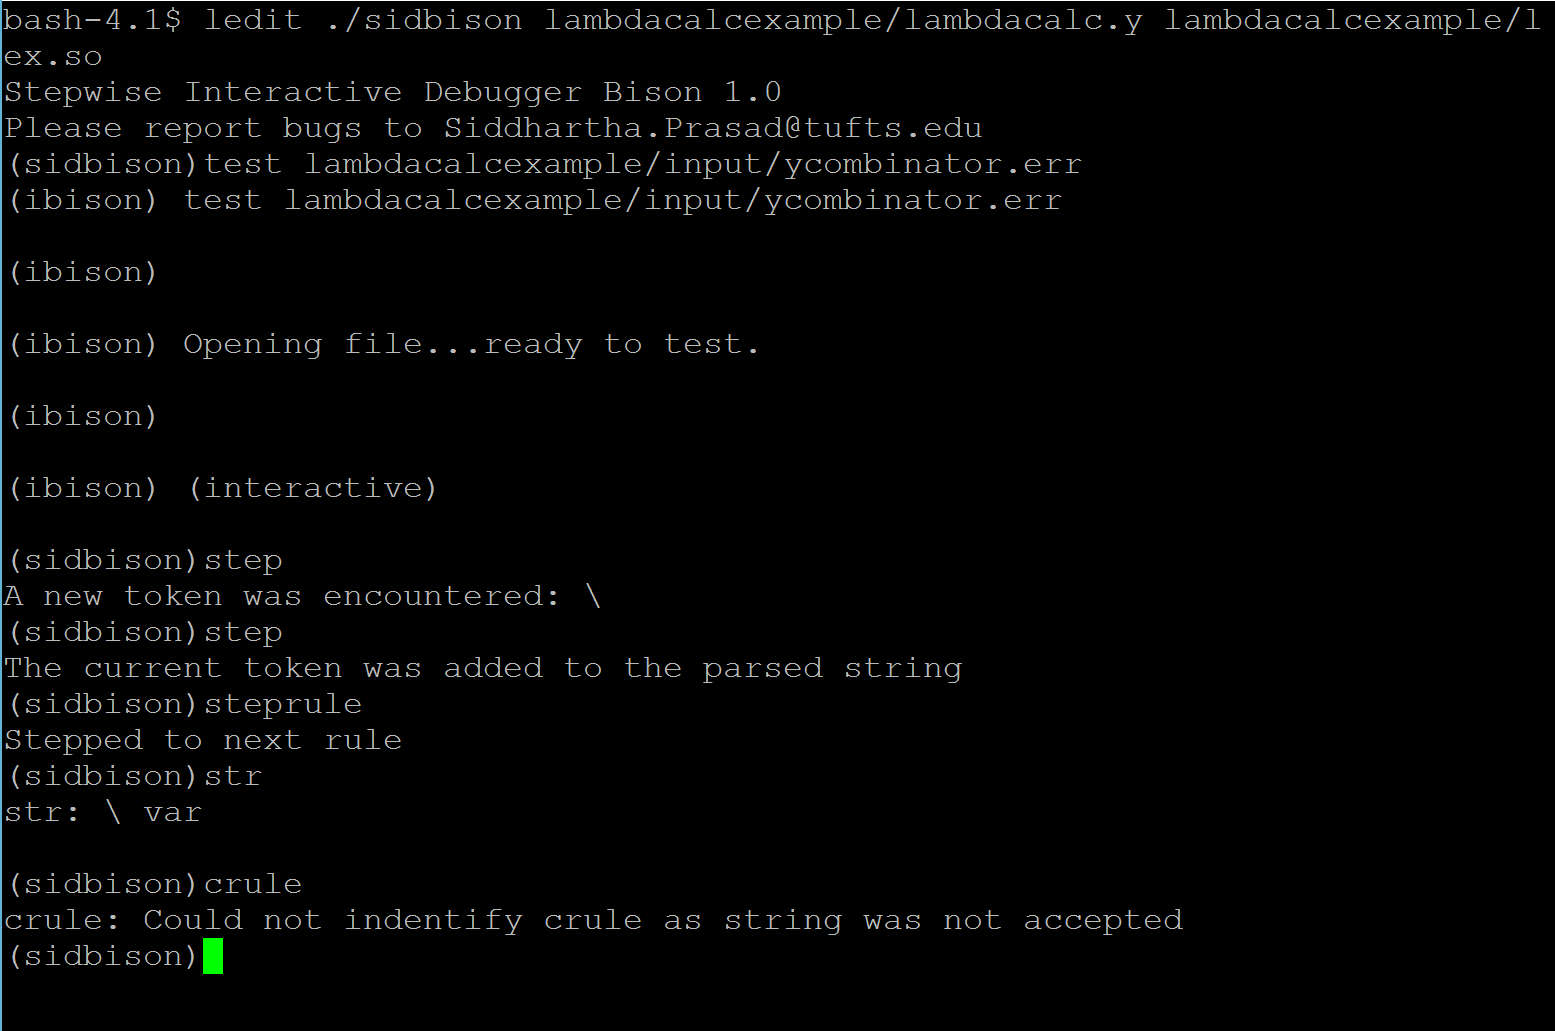
\includegraphics[width=10cm]{lc_2.png}
\end{figure}

\noindent

The \verb|step| command executes a single parser step. The first \verb|step| executes the action of \textit{looking ahead} to the
\verb|\| character. The \verb|steprule| command is then used to step to the next rule being parsed. The \verb|str| command shows that this rule was named \verb|var|. The current rule being parsed could not be identified since the entire string was not accepted. \verb|iBison| is trying to parse the entire subsequent string, alongside the current results of \verb|str| to a top level rule. However, the string does not match any rules in the grammar.

\begin{figure}[H] \centering
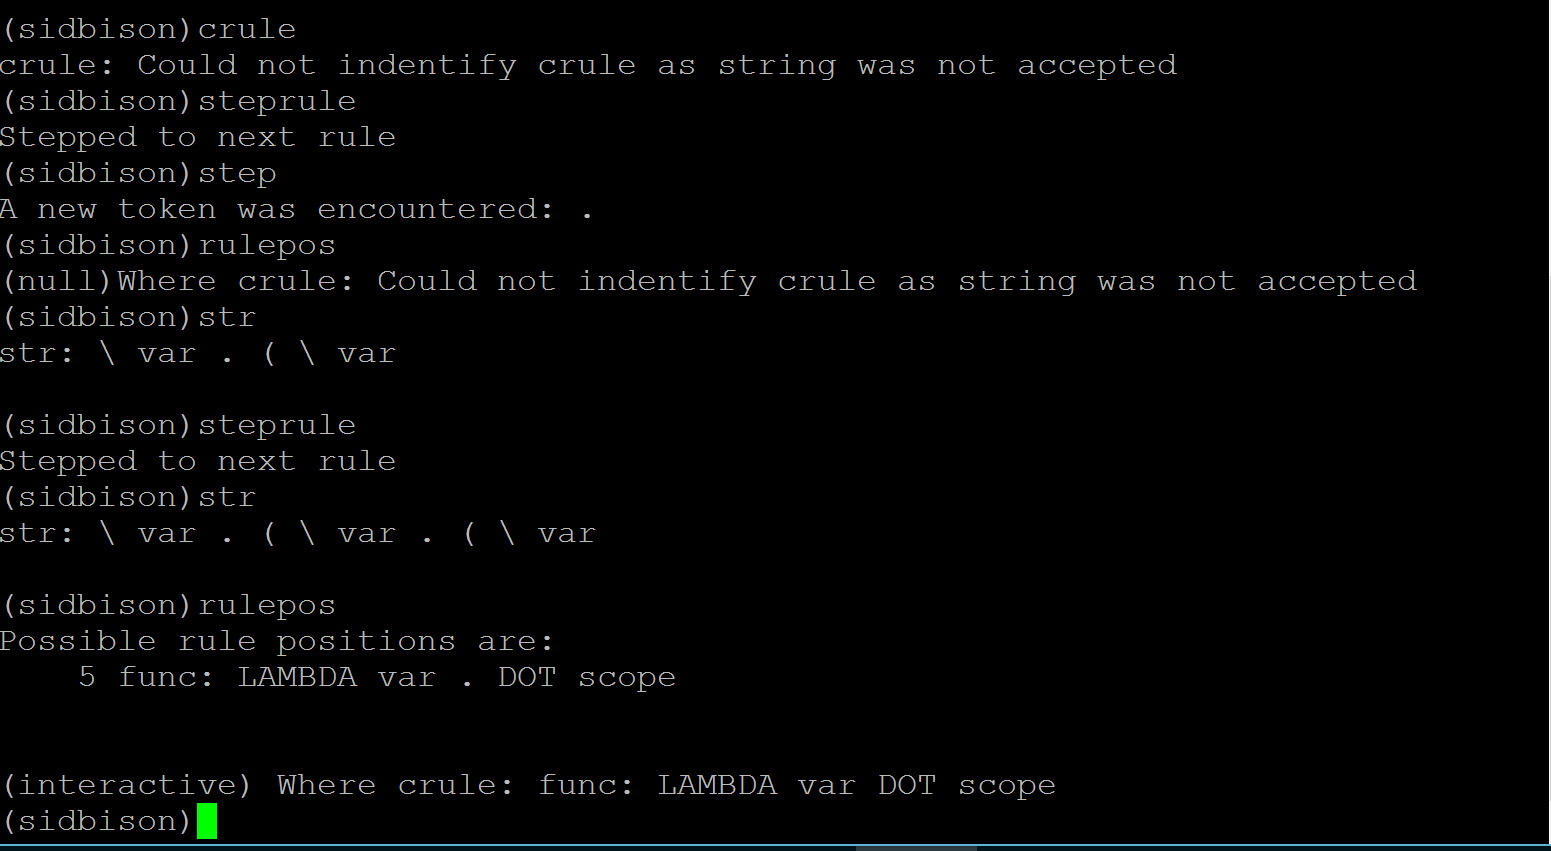
\includegraphics[width=10cm]{lc_3.png}
\end{figure}

\noindent

After stepping two more rules, the \verb|rulepos| rule uses a \verb|.| to show the current  position in the parsing process, as well as the current rule.

\begin{figure}[H] \centering
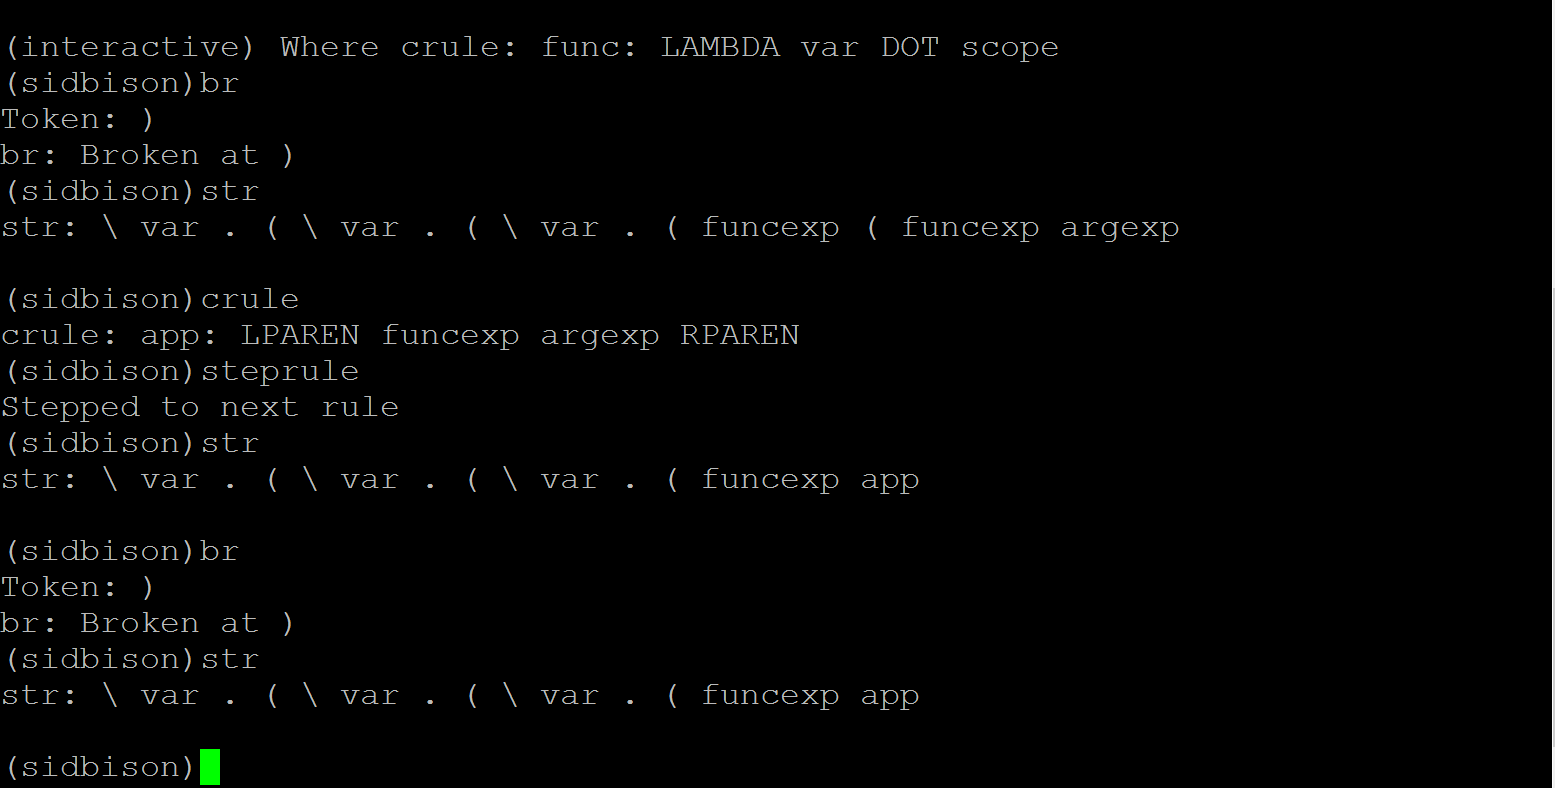
\includegraphics[width=10cm]{lc_4.png}
\end{figure}

\noindent
The \verb|break| command can be used to step forward till the current token being looked at is a \verb|)|. The \verb|str| command shows the current state in the parsing process.

\begin{figure}[H] \centering
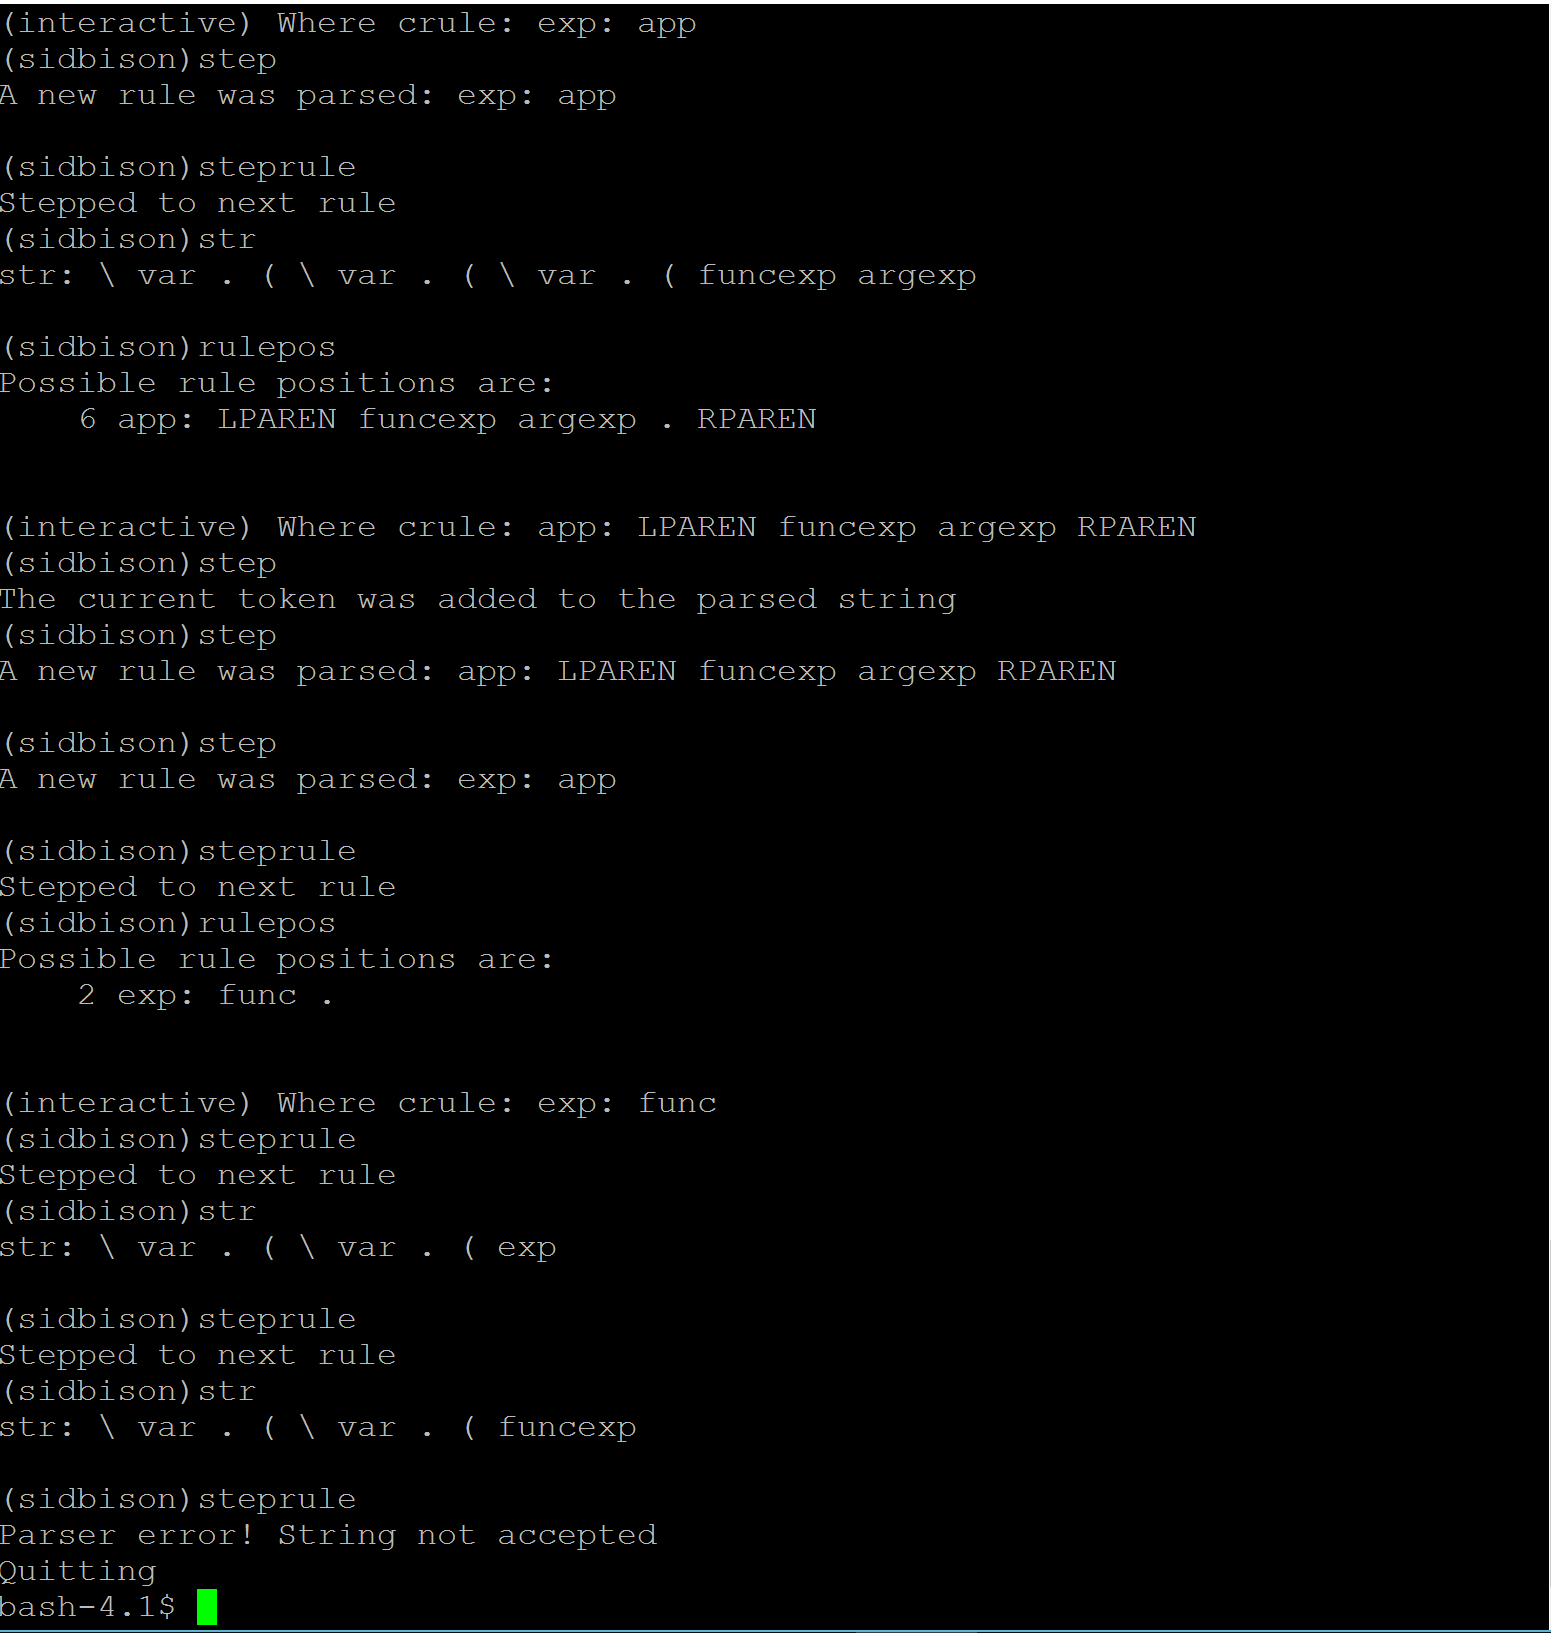
\includegraphics[width=10cm]{lc_5.png}
\end{figure}

\noindent

The parsing process reaches lower level rules. \verb||rulepos| and \verb|crule| show the current rules being parsed. The only rule that starts and ends with parentheses is observed to be \verb|app|. Thus, \verb|iBison| attempts to parse \verb|(\x.(h (x x)))| as a function application with no argument. As a result, \href{https://github.com/sidprasad/sidbison/blob/master/lambdacalcexample/input/ycombinator.err} {ycombinator.err} is not accepted.



\section{Impcore}

\section{Source Code}

Source code for \verb|sidBison| be found at \url{https://github.com/sidprasad/sidbison/}. 

\noindent
Example Flex and Bison specifications can be found in Appendix B.

\noindent
 Source code and instructions for building and installing iBison can be found at \url{https://www.cs.uic.edu/~spopuri/ibison.html}.